\documentclass[11pt,letterpaper]{article}
\usepackage[T1]{fontenc}
\usepackage{lmodern}
\usepackage[margin=1in]{geometry}
\usepackage{amsmath,amssymb,amsthm,mathtools}
\usepackage{enumitem}
\usepackage{microtype}
\usepackage{tikz}
\usepackage[colorlinks=true,linkcolor=blue,citecolor=blue,urlcolor=blue]{hyperref}
\usepackage{bookmark}
\pdftrailerid{}
\pdfsuppressptexinfo=15

\newtheorem{theorem}{Theorem}[section]
\newtheorem{proposition}[theorem]{Proposition}
\newtheorem{lemma}[theorem]{Lemma}
\newtheorem{corollary}[theorem]{Corollary}
\theoremstyle{definition}
\newtheorem{definition}[theorem]{Definition}
\theoremstyle{remark}
\newtheorem{remark}[theorem]{Remark}
\numberwithin{equation}{section}
\setlist{itemsep=3pt,topsep=5pt}
\hypersetup{pdftitle={Talagrand's discrete-convexity conjecture},
  pdfauthor={OpenAI},
  pdfsubject={A positive solution to Talagrand's Research Problem 13.3.2}}

\newcommand{\unverified}[1]{\par\smallskip\noindent\fbox{\parbox{0.95\linewidth}{\textbf{Unverified step.} #1}}\par\smallskip}
\newcommand{\step}[2]{\medskip\noindent\textbf{Step #1} (#2)\textbf{.}\ }

\title{Talagrand's discrete-convexity conjecture}
\author{Rewritten for readability from the OpenAI manuscript of the same title}
\date{September 23, 2026}

\AddToHook{cmd/thebibliography/after}{\addcontentsline{toc}{section}{\refname}}

\begin{document}
\maketitle
\begin{abstract}
We prove Talagrand's discrete-convexity conjecture.
There is a universal integer $k$ such that, whenever an arbitrary family has
Bernoulli product measure at least $1-1/k$, the sets not contained
in a union of $k$ members admit a cover of total cost at most $1/2$
at the same density. This version reorganises the argument so that every
step can be checked on its own; the statements, constants and proof
strategy are those of the original manuscript.
\end{abstract}

\section{The result and how it is proved}
\label{sec:introduction}

\subsection{Setting}

Throughout, $N\ge1$ is an integer, $[N]=\{1,\ldots,N\}$, and a
\emph{family} is a subset of $2^{[N]}$. For $p\in(0,1)$, $\mu_p$ is the
probability measure on $2^{[N]}$ under which each element of $[N]$ is
present independently with probability $p$; that is,
$\mu_p(\{S\})=p^{|S|}(1-p)^{N-|S|}$.

\paragraph{Exceptional sets.}
For a family $\mathcal D$ and an integer $k\ge1$, the family
$E_k(\mathcal D)$ consists of the sets that \emph{cannot} be covered by
$k$ members of $\mathcal D$:
\begin{equation}
\label{eq:exceptional-definition}
S\in E_k(\mathcal D)
\iff
\text{there is no tuple }(D_1,\ldots,D_k)\in\mathcal D^k
\text{ with }S\subseteq D_1\cup\cdots\cup D_k .
\end{equation}
The members of a tuple may repeat and need not be disjoint. Two facts
follow at once from the definition and are used later.
\begin{itemize}
\item If $\mathcal D\neq\varnothing$, then $\varnothing\notin E_k(\mathcal D)$,
because $\varnothing\subseteq D\cup\cdots\cup D$ for any $D\in\mathcal D$.
\item $E_k(\mathcal D)$ is increasing: if $S\in E_k(\mathcal D)$ and
$S\subseteq S'$, then $S'\in E_k(\mathcal D)$, because a union containing
$S'$ would contain $S$.
\end{itemize}

\paragraph{Covers and smallness.}
A family $\mathcal G$ \emph{covers} a family $\mathcal A$ if every
$S\in\mathcal A$ contains some $I\in\mathcal G$. The members of
$\mathcal G$ are called \emph{generators}. For $\rho\in(0,1)$ the
\emph{cost of $\mathcal G$ at density $\rho$} is
\[
c_\rho(\mathcal G)=\sum_{I\in\mathcal G}\rho^{|I|}.
\]
A family $\mathcal A$ is \emph{$\rho$-small} if it has a cover
$\mathcal G$ with $c_\rho(\mathcal G)\le1/2$. Three remarks:
\begin{itemize}
\item Since $\mu_p\{S:I\subseteq S\}=p^{|I|}$, a cover $\mathcal G$ of
$\mathcal A$ gives $\mu_p(\mathcal A)\le c_p(\mathcal G)$ by a union bound.
So $p$-smallness is an explicit certificate that $\mu_p(\mathcal A)\le1/2$.
\item $c_\rho(\mathcal G)$ is nondecreasing in $\rho$. Hence
$\rho$-small implies $\rho'$-small for every $\rho'\le\rho$:
smallness at a \emph{lower} density is a \emph{weaker} statement.
\item The empty family $\mathcal A=\varnothing$ is covered by
$\mathcal G=\varnothing$ at cost $0$.
\end{itemize}

\paragraph{A toy example.}
Let $N=3$, $\mathcal D=\{\{1\},\{2\}\}$, $k=2$. The unions of two members
are $\{1\},\{2\},\{1,2\}$, so $E_2(\mathcal D)=\{S:3\in S\}$. It is
covered by $\mathcal G=\{\{3\}\}$, whose cost at density $p$ is $p$.

\subsection{The main theorem}

Talagrand formulated the discrete-convexity conjecture in
\cite[Conjecture~7.1]{Talagrand10}: a fixed number of members of a
sufficiently likely family should cover every set outside a $p$-small
exceptional family. The same formulation, at the original density $p$,
appears as Research Problem~13.3.2 in~\cite{Talagrand21}. The following
theorem proves it.

\begin{theorem}
\label{thm:main}
Set $k=2^{75}$. For every integer $N\ge1$, every $p\in(0,1)$, and every
family $\mathcal D\subseteq2^{[N]}$,
\[
\mu_p(\mathcal D)\ge1-\frac1k
\quad\Longrightarrow\quad
E_k(\mathcal D)\text{ is }p\text{-small}.
\]
\end{theorem}

The constant is independent of $N$, $p$, and $\mathcal D$.
The family $\mathcal D$ is arbitrary; no monotonicity is assumed.
The measure in the hypothesis and the density in the conclusion are the
same $p$.

\subsection{Proof at a glance}
\label{sec:glance}

\paragraph{Key idea.}
Fix a family $\mathcal F$ and a density $q$ with $\mu_q(\mathcal F)\ge1/2$.
To every $U\subseteq[N]$ we attach a weight $w(U)\ge0$ (a rescaled squared
Fourier coefficient of the indicator of $\mathcal F$) with two properties.
\begin{itemize}
\item[(W1)] \emph{Globally the weights are small:}
$\sum_{U\subseteq[N]}q^{|U|}w(U)\le1$. This is Parseval's identity.
\item[(W2)] \emph{On every exceptional set they are large:}
every $S\in E_{32}(\mathcal F)$ satisfies
$\sum_{\varnothing\ne U\subseteq S}w(U)^{16}\ge2^{-32}$. This comes from a
signed measure on $32\times N$ arrays that vanishes unless the $32$ rows
jointly cover $S$.
\end{itemize}
By (W2), an exceptional set must contain either one subset $U$ of large
weight, or very many subsets of the same size and comparable smaller
weight. By (W1), the subsets of large weight are cheap to use as
generators, and each class of ``same size, comparable weight'' has bounded
total cost. A separate combinatorial lemma covers, cheaply, all sets
containing very many members of such a class.

\paragraph{The steps and their dependencies.}
\begin{enumerate}
\item \textbf{Lemma~\ref{lem:covering}} (Section~\ref{sec:covering}),
a self-contained covering lemma. If an $r$-uniform family $\mathcal H$ has
$|\mathcal H|\rho^r\le2^{h+1}$, then the sets containing at least $2^{12h}$
members of $\mathcal H$ have a cover of cost at most $3\cdot2^{-h}$ at
density $\rho$. The proof is a random construction.
\item \textbf{Proposition~\ref{prop:half-density}}
(Section~\ref{sec:weights}). If $\mu_q(\mathcal F)\ge1/2$, then
$E_{32}(\mathcal F)$ is $(q/2^{70})$-small. It proves (W1) and (W2), takes
the heavy sets as generators, sorts the others into bins by size $r$ and by
dyadic weight scale $2^{-h}$, and applies Lemma~\ref{lem:covering} to each
bin. A set that avoids all generators contains fewer than $2^{12h}$ sets of
each bin, each contributing at most $2^{-16h}$ to the sum in (W2), so the
sum is below $2^{-32}$ and the set is not exceptional. The sixteenth power
is what makes $2^{12h}\cdot2^{-16h}=2^{-4h}$ summable.
\item \textbf{Proof of Theorem~\ref{thm:main}} (Section~\ref{sec:density}).
Step~2 loses a factor $L=2^{70}$ in the density. To undo this, take
$L$ random sets $R_1,\ldots,R_L$, each with law exactly $\mu_p$, coupled so
that they are pairwise disjoint; their union then has law $\mu_{Lp}$.
Apply step~2 with $q=Lp$ to the family $\mathcal F$ of unions of $L$
members of $\mathcal D$. Then $E_{32}(\mathcal F)=E_{32L}(\mathcal D)$ and
$q/L=p$. This needs $Lp<1$; when $Lp\ge1$ a different coupling shows
directly that $E_k(\mathcal D)=\varnothing$.
\end{enumerate}

\begin{center}
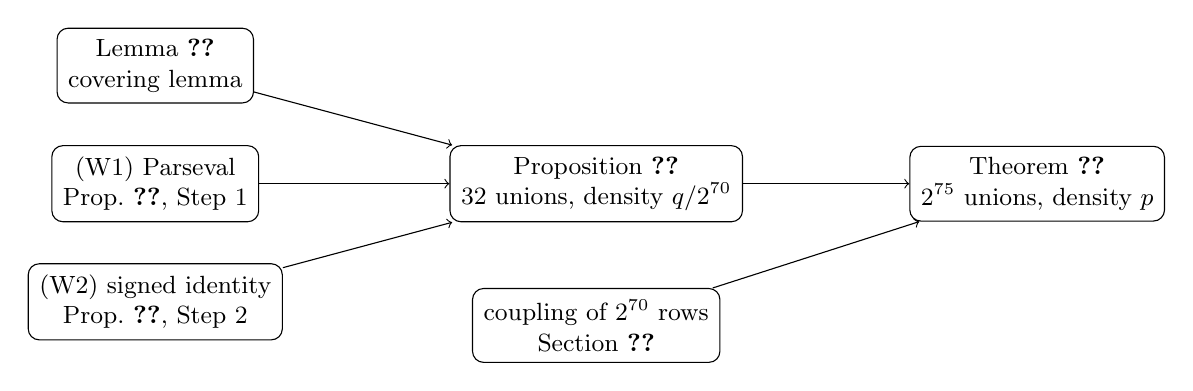
\begin{tikzpicture}[box/.style={draw,rounded corners,align=center,inner sep=4pt,font=\small}]
\node[box] (lem) at (0,0) {Lemma~\ref{lem:covering}\\ covering lemma};
\node[box] (w1) at (0,-1.5) {(W1) Parseval\\ Prop.~\ref{prop:half-density}, Step 1};
\node[box] (w2) at (0,-3.0) {(W2) signed identity\\ Prop.~\ref{prop:half-density}, Step 2};
\node[box] (prop) at (5.6,-1.5) {Proposition~\ref{prop:half-density}\\ $32$ unions, density $q/2^{70}$};
\node[box] (cpl) at (5.6,-3.3) {coupling of $2^{70}$ rows\\ Section~\ref{sec:density}};
\node[box] (thm) at (11.2,-1.5) {Theorem~\ref{thm:main}\\ $2^{75}$ unions, density $p$};
\draw[->] (lem) -- (prop);
\draw[->] (w1) -- (prop);
\draw[->] (w2) -- (prop);
\draw[->] (prop) -- (thm);
\draw[->] (cpl) -- (thm);
\end{tikzpicture}
\end{center}

\paragraph{Where the constants come from.}
$k=32\cdot2^{70}$. The $32$ is the number of rows in (W2), giving the
exponent $32=2\cdot16$. The factor $2^{70}=2^{64}\cdot2^{6}$ arises in
Proposition~\ref{prop:half-density}: the threshold $2^{-64|U|}$ for
``heavy'' sets guarantees that every bin has $h\ge64$, as
Lemma~\ref{lem:covering} requires, and the extra $2^{-6}$ makes the heavy
generators cost at most $1/64$.

\paragraph{What is not on the path to Theorem~\ref{thm:main}.}
Section~\ref{sec:context} collects a consequence for positive selector
processes, a two-union corollary that depends on external results, and
pointers to related work. None of it is used in
Sections~\ref{sec:covering}--\ref{sec:density}.

\paragraph{Notation changes relative to the original manuscript.}
To keep one meaning per symbol, a few letters are renamed. The signed
column mass in Section~\ref{sec:weights} is $\widetilde P$ (originally
$R$, which clashes with the random rows $R_j$). The random point of the
cube in Section~\ref{sec:weights} is $\xi$ (originally $X$, which clashes
with the ground set of Lemma~\ref{lem:covering}). The inclusion
probability in Case~2 of Section~\ref{sec:density} is $\tau$
(originally $t$). In Section~\ref{sec:context} the selector class is
$\mathcal T$ with elements $\theta$ (originally $T$ and $t$), and the
density in the two-union corollary is $\sigma$ (originally $r$).
In Section~\ref{sec:covering}, $\pi$ is a probability, not the circle
constant, and $e,e'$ are edges, so the exponential is written $\exp$.

\section{An elementary covering lemma}
\label{sec:covering}

\paragraph{Where this is used.}
Only in Step~4 of the proof of Proposition~\ref{prop:half-density}, with
$X=[N]$, $\rho=q/2^{70}$, and $\mathcal H$ a bin of sets of size $r$ whose
weights are about $2^{-h}$.

\paragraph{What it says.}
Think of $\rho^r$ as the cost of one member (``edge'') of an $r$-uniform
family $\mathcal H$. The total cost $|\mathcal H|\rho^r$ may be as large as
$2^{h+1}$, so the edges themselves are far too expensive to serve as
generators. The lemma says that the sets containing a huge number,
$2^{12h}$, of edges can nevertheless be covered at tiny cost.
Unions of sampled edges also appear in the covering constructions of
Fischer and Person \cite[Sections~1.1 and~2]{FischerPerson25}; the argument
below is self-contained.

\begin{lemma}\label{lem:covering}
Let \(X\) be a finite set, let \(0<\rho<1\), and let \(r,h\) be integers
with \(1\le r\le h\) and \(h\ge64\). Suppose that
\(\mathcal H\subseteq\binom{X}{r}\) satisfies
\[
|\mathcal H|\rho^r\le2^{h+1}.
\]
Then the family
\[
\left\{S\subseteq X:
  |\{e\in\mathcal H:e\subseteq S\}|\ge2^{12h}\right\}
\]
has a cover \(\mathcal G\subseteq2^X\) with
\[
c_\rho(\mathcal G)\le3\cdot2^{-h}.
\]
\end{lemma}

\begin{proof}
\emph{Plan.} We build $\mathcal G=\mathcal C_0\cup\mathcal C_1\cup\mathcal C_2$.
The part $\mathcal C_0$ is deterministic; $\mathcal C_1$ and $\mathcal C_2$
depend on a random sample. We show that $\mathcal G$ is a cover for
\emph{every} outcome of the sample (Step~4) and that its \emph{expected}
cost is at most $3\cdot2^{-h}$ (Steps~1, 3, 5). Some outcome then has cost
at most the expectation (Step~6).

Call the family in the statement the \emph{target family}. Put
\[
m=2^{12h},\qquad T=2^{4h},\qquad \pi=2^{-8h},
\qquad\text{so that}\qquad \pi m=2^{4h}.
\]

\step{1}{sets of large weighted degree: the generators $\mathcal C_0$}
For \(I\subseteq X\) with \(|I|\le r\), define the weighted degree
\[
d(I)=|\{e\in\mathcal H:I\subseteq e\}|\,\rho^{r-|I|}.
\]
Thus $d(I)\rho^{|I|}$ is the total cost $\rho^r$ of the edges containing
$I$, and $d(I)>T$ means that $I$ is more than $T$ times cheaper than the
edges through it. Let
\[
\mathcal C_0=\{I\subseteq X:|I|\le r,\ d(I)>T\}.
\]
Exchanging the order of summation, and using that each edge has exactly
$2^r$ subsets,
\[
\sum_{\substack{I\subseteq X\\|I|\le r}}d(I)\rho^{|I|}
=\sum_{I}\ \sum_{\substack{e\in\mathcal H\\ e\supseteq I}}\rho^{r}
=\rho^r\sum_{e\in\mathcal H}|\{I:I\subseteq e\}|
=2^r|\mathcal H|\rho^r.
\]
For $I\in\mathcal C_0$ we have $1<d(I)/T$. Therefore
\begin{equation}\label{eq:covering-initial-cost}
c_\rho(\mathcal C_0)=\sum_{I\in\mathcal C_0}\rho^{|I|}
\le\frac1T\sum_{I\in\mathcal C_0}d(I)\rho^{|I|}
\le\frac{2^r|\mathcal H|\rho^r}{T}
\le2^{-4h}\cdot2^r\cdot2^{h+1}=2^{r+1-3h}\le2^{1-2h}.
\end{equation}
The third inequality is the hypothesis $|\mathcal H|\rho^r\le2^{h+1}$;
the last uses $r\le h$.

\step{2}{regular edges and the extension inequality}
Call an edge $e\in\mathcal H$ \emph{regular} if it contains no member of
\(\mathcal C_0\), and let \(\mathcal H'\) be the family of regular edges.
Since every subset of an edge has size at most $r$, the definition of
$\mathcal C_0$ gives
\begin{equation}\label{eq:regular}
I\subseteq e\ \text{ for some }e\in\mathcal H'
\quad\Longrightarrow\quad d(I)\le T.
\end{equation}

\emph{Claim.} For every \(B\subseteq X\),
\begin{equation}\label{eq:covering-extension}
\sum_{e\in\mathcal H'}\rho^{|e\setminus B|}
\le T\sum_{i=0}^r\binom{|B|}{i}.
\end{equation}

\emph{Proof of the claim.} Sort the regular edges $e$ according to the set
$I=e\cap B$. This $I$ is a subset of $B$ of size at most $r$, so there are
at most $\sum_{i=0}^r\binom{|B|}{i}$ possible values of $I$. Fix an $I$ for
which the group $\{e\in\mathcal H':e\cap B=I\}$ is nonempty. Every $e$ in
the group has $|e\setminus B|=r-|I|$ and contains $I$, so
\[
\sum_{\substack{e\in\mathcal H'\\e\cap B=I}}
  \rho^{|e\setminus B|}
=|\{e\in\mathcal H':e\cap B=I\}|\,\rho^{r-|I|}
\le|\{e\in\mathcal H:I\subseteq e\}|\,\rho^{r-|I|}
= d(I)\le T.
\]
The last inequality is \eqref{eq:regular}, which applies because the group
is nonempty. Summing over the possible $I$ gives
\eqref{eq:covering-extension}.

\step{3}{sampled pairs: the generators $\mathcal C_1$}
Independently for each ordered pair \((e,e')\in(\mathcal H')^2\),
including the diagonal pairs $(e,e)$, \emph{sample} that pair with
probability \(\pi\). Let \(\mathcal C_1\) be the set of unions $e\cup e'$
of sampled pairs.

Each member of $\mathcal C_1$ is the union of at least one sampled pair, so
$c_\rho(\mathcal C_1)\le\sum_{(e,e')\text{ sampled}}\rho^{|e\cup e'|}$.
Here a union arising from several sampled pairs is counted several
times on the right. Taking expectations (linearity only; independence is not
used here),
\begin{align}
\mathbb E[c_\rho(\mathcal C_1)]
&\le\pi\sum_{(e,e')\in(\mathcal H')^2}\rho^{|e\cup e'|}
=\pi\sum_{e\in\mathcal H'}\rho^{r}\sum_{e'\in\mathcal H'}\rho^{|e'\setminus e|}
\notag\\
&\le\pi\,|\mathcal H'|\,\rho^r\,2^rT
\le2^{-8h}\cdot2^{h+1}\cdot2^r\cdot2^{4h}
=2^{r+1-3h}\le2^{1-2h}.
\label{eq:covering-pair-cost}
\end{align}
The equality uses $|e\cup e'|=|e|+|e'\setminus e|=r+|e'\setminus e|$. The
next inequality is \eqref{eq:covering-extension} with $B=e$, where $|B|=r$
and $\sum_{i=0}^r\binom ri=2^r$. Then we use
$|\mathcal H'|\rho^r\le|\mathcal H|\rho^r\le2^{h+1}$ and finally $r\le h$.

\step{4}{residual tuples: the generators $\mathcal C_2$; $\mathcal G$ is always a cover}
For every ordered tuple \((e_1,\ldots,e_m)\) of \emph{distinct} regular
edges, put \(e_1\cup\cdots\cup e_m\) into \(\mathcal C_2\) if none of the
$m^2$ pairs \((e_i,e_j)\), \(1\le i,j\le m\) (including $i=j$), was sampled.
Set
\[
\mathcal G=\mathcal C_0\cup\mathcal C_1\cup\mathcal C_2 .
\]
We check that $\mathcal G$ covers the target family for every sampling
outcome. Let $S$ be a target set. If $S$ contains a member of
$\mathcal C_0$, we are done. Otherwise every edge $e\in\mathcal H$ with
$e\subseteq S$ is regular: a member of $\mathcal C_0$ inside $e$ would lie
inside $S$. Since $S$ is a target set, it contains at least $m$ edges, all
regular; choose $m$ distinct ones and order them as $(e_1,\ldots,e_m)$. If
some pair $(e_i,e_j)$ was sampled, then $e_i\cup e_j\in\mathcal C_1$ and
$e_i\cup e_j\subseteq S$. If no such pair was sampled, then
$e_1\cup\cdots\cup e_m\in\mathcal C_2$ and it is contained in $S$.

\step{5}{expected cost of $\mathcal C_2$}

\emph{5a. Total weight of tuples.} For \(0\le t\le m\), let
\[
W_t=
\sum_{\substack{(e_1,\ldots,e_t)\in(\mathcal H')^t\\
                e_1,\ldots,e_t\ \text{distinct}}}
  \rho^{|e_1\cup\cdots\cup e_t|},
\qquad W_0=1
\]
(for $t=0$ there is one empty tuple, with empty union). We claim
\begin{equation}\label{eq:W-recursion}
W_{t+1}\le T(1+rm)^r\,W_t\quad(0\le t<m),
\qquad\text{hence}\qquad
W_m\le\bigl[T(1+rm)^r\bigr]^m .
\end{equation}
Fix a tuple $(e_1,\ldots,e_t)$ of distinct regular edges with $t<m$ and let
$B=e_1\cup\cdots\cup e_t$, so $|B|\le rt\le rm$. First,
\[
\sum_{i=0}^r\binom{|B|}{i}\le(1+|B|)^r\le(1+rm)^r .
\]
To see the first inequality, fix a linear order on $B$ and a new symbol
$\ast$. Map a subset $\{b_1<\cdots<b_i\}$ of $B$ with $i\le r$ to the
sequence $(b_1,\ldots,b_i,\ast,\ldots,\ast)$ of length $r$; this is an
injection into $(B\cup\{\ast\})^r$. Second, for any edge $e$ we have
\(\rho^{|B\cup e|}=\rho^{|B|}\rho^{|e\setminus B|}\). Hence, by
\eqref{eq:covering-extension},
\[
\sum_{e\in\mathcal H'\setminus\{e_1,\ldots,e_t\}}\rho^{|B\cup e|}
\le\rho^{|B|}\sum_{e\in\mathcal H'}\rho^{|e\setminus B|}
\le\rho^{|B|}\,T(1+rm)^r .
\]
(Allowing all regular edges $e$, not only the new ones, can only increase
the sum.) Summing over all tuples $(e_1,\ldots,e_t)$ gives the recursion in
\eqref{eq:W-recursion}. Iterating from $W_0=1$ gives the bound on $W_m$.

\emph{5b. Survival probability of one tuple.} Fix a tuple
$(e_1,\ldots,e_m)$ of distinct regular edges. Because the $e_i$ are
distinct, the $m^2$ ordered pairs $(e_i,e_j)$ are $m^2$ \emph{different}
elements of $(\mathcal H')^2$. These pairs are sampled independently, so
the probability that none of them is sampled is exactly
\[
(1-\pi)^{m^2}\le \exp(-\pi m^2)\le2^{-\pi m^2}.
\]
Here $1-\pi\le\exp(-\pi)$, and $\exp(-x)\le2^{-x}$ for $x\ge0$ because
$\ln2<1$. This is the only place where independence of the sample is used.

\emph{5c. Expected cost.} Each member of $\mathcal C_2$ is the union of at
least one tuple none of whose pairs was sampled. Counting with
multiplicity as in Step~3 and using linearity of expectation together
with 5a and 5b,
\[
\mathbb E[c_\rho(\mathcal C_2)]
\le W_m\,(1-\pi)^{m^2}
\le\bigl[T(1+rm)^r\bigr]^m\,2^{-\pi m^2}.
\]
We now show that the right side is at most $2^{-m}$. Using $r\le h$ and
$h+1\le2^h$,
\[
1+rm\le1+h\,2^{12h}\le(h+1)2^{12h}\le2^{13h},
\qquad\text{so}\qquad
\log_2\bigl[T(1+rm)^r\bigr]\le4h+13rh .
\]
Next, using $r\le h$, then $4h+1\le5h\le5h^2$, then $h\le2^h$, and finally
$18\le2^{2h}$ (true for $h\ge3$, and we have $h\ge64$),
\[
4h+13rh+1\le4h+13h^2+1\le18h^2\le18\cdot2^{2h}\le2^{4h}=\pi m .
\]
Multiplying $4h+13rh\le\pi m-1$ by $m$ gives
$(4h+13rh)m-\pi m^2\le-m$. It follows that
\begin{equation}\label{eq:covering-residual-cost}
\mathbb E[c_\rho(\mathcal C_2)]
\le2^{(4h+13rh)m-\pi m^2}\le2^{-m}.
\end{equation}

\step{6}{conclusion}
Since $c_\rho(\mathcal G)\le c_\rho(\mathcal C_0)+c_\rho(\mathcal C_1)
+c_\rho(\mathcal C_2)$, the bounds \eqref{eq:covering-initial-cost},
\eqref{eq:covering-pair-cost}, and \eqref{eq:covering-residual-cost} give
\[
\mathbb E[c_\rho(\mathcal G)]
\le2^{1-2h}+2^{1-2h}+2^{-m}=2^{2-2h}+2^{-m}\le2^{-h}+2^{-h}\le3\cdot2^{-h}.
\]
Here $2^{2-2h}\le2^{-h}$ because $h\ge2$, and $2^{-m}\le2^{-h}$ because
$m=2^{12h}\ge h$. The sample space is finite, so some outcome has
$c_\rho(\mathcal G)$ at most its expectation. By Step~4 that outcome's
$\mathcal G$ is a cover of the target family.
\end{proof}

\section{Weights for exceptional sets}
\label{sec:weights}

This section proves the theorem with a fixed loss $L=2^{70}$ in the
density and only $32$ unions. It is used once, in Case~1 of the proof of
Theorem~\ref{thm:main}.

\begin{proposition}\label{prop:half-density}
Let $L=2^{70}$. For every integer $N\ge1$, every $q\in(0,1)$, and every
$\mathcal F\subseteq 2^{[N]}$ satisfying $\mu_q(\mathcal F)\ge1/2$,
the family $E_{32}(\mathcal F)$ is $(q/L)$-small.
\end{proposition}

\begin{proof}
\emph{Plan.} We define weights $w(U)$ and prove the global bound (W1) in
Step~1 and the local bound (W2) in Step~2. Steps~3--5 build a cover from
the heavy sets and from Lemma~\ref{lem:covering} applied to bins of lighter
sets, and bound its cost. Step~6 shows that it covers
$E_{32}(\mathcal F)$ by comparing (W2) with a count over bins.

\paragraph{Notation.}
Identify a subset of $[N]$ with its indicator vector in $\{0,1\}^N$, and
write $f=\mathbf 1_{\mathcal F}:\{0,1\}^N\to\{0,1\}$. For
$U\subseteq[N]$, $z\in\{0,1\}^U$ and $y\in\{0,1\}^{[N]\setminus U}$, write
$(z,y)$ for the point of $\{0,1\}^N$ that agrees with $z$ on $U$ and with
$y$ off $U$. Define
\begin{equation}\label{eq:weights-definition}
 b(U)=(1-q)^{|U|}
 \sum_{z\in\{0,1\}^{U}}(-1)^{\sum_{i\in U}z_i}\,
 \mathbb E[f(z,Y)],
 \qquad w(U)=b(U)^2\ge0,
\end{equation}
where $Y$ is a random element of $\{0,1\}^{[N]\setminus U}$ with
independent Bernoulli-$q$ coordinates. For $U=\varnothing$ the sum has
one term and
\begin{equation}\label{eq:b-empty}
b(\varnothing)=\mathbb E[f(Y)]=\mu_q(\mathcal F)\ge\tfrac12 .
\end{equation}

\step{1}{the global weight bound \textup{(W1)}}
We show
\begin{equation}\label{eq:global-weight-bound}
 \sum_{U\subseteq[N]}q^{|U|}w(U)\le1 .
\end{equation}
We use the standard biased Fourier basis
\cite[Section~8.4]{ODonnell14}, with the normalization made explicit.
Let $\xi=(\xi_1,\ldots,\xi_N)$ have law $\mu_q$, and for $x\in\{0,1\}^N$
put
\[
 g_i(x)=\frac{q-x_i}{\sqrt{q(1-q)}},\qquad
 \chi_U(x)=\prod_{i\in U}g_i(x)
 =\frac{\prod_{i\in U}(q-x_i)}{[q(1-q)]^{|U|/2}},
 \qquad U\subseteq[N].
\]

\emph{1a. Orthonormality.}
$\mathbb E[g_i(\xi)]=\bigl((1-q)q+q(q-1)\bigr)/\sqrt{q(1-q)}=0$ and
$\mathbb E[g_i(\xi)^2]=\bigl((1-q)q^2+q(1-q)^2\bigr)/(q(1-q))=1$.
By independence of the coordinates,
\[
\mathbb E[\chi_U(\xi)\chi_V(\xi)]
=\prod_{i\in U\cap V}\mathbb E[g_i(\xi)^2]
 \prod_{i\in U\triangle V}\mathbb E[g_i(\xi)]
=\begin{cases}1,&U=V,\\0,&U\ne V.\end{cases}
\]
Since $0<q<1$, $\mu_q$ has full support, so
$\langle g,g'\rangle=\mathbb E[g(\xi)g'(\xi)]$ is an inner product on the
$2^N$-dimensional space of real functions on $\{0,1\}^N$. The $2^N$
orthonormal functions $\chi_U$ therefore form an orthonormal basis. With
$\widehat f(U)=\mathbb E[f(\xi)\chi_U(\xi)]$, Parseval's identity reads
\begin{equation}\label{eq:parseval}
\sum_{U\subseteq[N]}\widehat f(U)^2=\mathbb E[f(\xi)^2].
\end{equation}

\emph{1b. Relation between $\widehat f$ and $b$.}
For one coordinate and $z_i\in\{0,1\}$,
\[
 \mathbb P(\xi_i=z_i)\,(q-z_i)=q(1-q)(-1)^{z_i},
\]
since $z_i=0$ gives $(1-q)\cdot q$ and $z_i=1$ gives $q\cdot(q-1)$.
Now condition on the restriction of $\xi$ to $U$ being $z$. The function
$\chi_U$ depends only on the coordinates in $U$, and the remaining
coordinates are independent of them with the law of $Y$. So
\[
 \widehat f(U)
 =\sum_{z\in\{0,1\}^U}\ \prod_{i\in U}
 \frac{\mathbb P(\xi_i=z_i)(q-z_i)}{\sqrt{q(1-q)}}\ \mathbb E[f(z,Y)]
 =[q(1-q)]^{|U|/2}
 \sum_{z\in\{0,1\}^{U}}(-1)^{\sum_{i\in U}z_i}\,
 \mathbb E[f(z,Y)] .
\]
Comparing with \eqref{eq:weights-definition},
\[
\widehat f(U)=\frac{[q(1-q)]^{|U|/2}}{(1-q)^{|U|}}\,b(U)
=\left(\frac{q}{1-q}\right)^{|U|/2}b(U),
\qquad\text{i.e.}\qquad
q^{|U|}w(U)=(1-q)^{|U|}\,\widehat f(U)^2 .
\]

\emph{1c. Conclusion.} Using 1b, then $(1-q)^{|U|}\le1$, then
\eqref{eq:parseval}, then $f^2=f$,
\[
 \sum_{U\subseteq[N]}q^{|U|}w(U)
 =\sum_{U\subseteq[N]}(1-q)^{|U|}\widehat f(U)^2
 \le\sum_{U\subseteq[N]}\widehat f(U)^2
 =\mathbb E[f(\xi)^2]
 =\mu_q(\mathcal F)\le1 .
\]

\step{2}{a lower bound on every exceptional set \textup{(W2)}}
Fix $S\in E_{32}(\mathcal F)$. We show
\begin{equation}\label{eq:exceptional-weight-bound}
 \sum_{\varnothing\ne U\subseteq S}w(U)^{16}\ge2^{-32}.
\end{equation}

\emph{2a. A signed measure on arrays.}
Consider arrays $\mathbf x=(x_{ji})\in\{0,1\}^{32\times N}$ with $32$ rows
and $N$ columns. Write $x_j\in\{0,1\}^N$ for row $j$ (a subset of $[N]$)
and $x^i\in\{0,1\}^{32}$ for column $i$. For a column
$y\in\{0,1\}^{32}$ let
\[
 P(y)=\prod_{j=1}^{32}q^{y_j}(1-q)^{1-y_j},
 \qquad
 \widetilde P(y)=P(y)-(1-q)^{32}(-1)^{\sum_{j=1}^{32}y_j}.
\]
$P$ is the mass function of $32$ independent Bernoulli-$q$ bits.
$\widetilde P$ is a signed correction of $P$, chosen so that
\begin{equation}\label{eq:zero-column}
\widetilde P(0,\ldots,0)=(1-q)^{32}-(1-q)^{32}=0,
\end{equation}
and so that the correction term is a product over the $32$ rows.
Define the signed weight of an array by
\[
\nu_S(\mathbf x)=\prod_{i\notin S}P(x^i)\ \prod_{i\in S}\widetilde P(x^i).
\]

\emph{2b. A vanishing sum.} We claim
\begin{equation}\label{eq:vanishing}
 \Sigma:=\sum_{\mathbf x\in\{0,1\}^{32\times N}}\nu_S(\mathbf x)
 \prod_{j=1}^{32}f(x_j)=0 .
\end{equation}
Indeed, every term is zero. If $\nu_S(\mathbf x)\ne0$, then by
\eqref{eq:zero-column} no column $x^i$ with $i\in S$ is all-zero, so every
$i\in S$ lies in some row: $S\subseteq x_1\cup\cdots\cup x_{32}$. By the
definition \eqref{eq:exceptional-definition} of $E_{32}(\mathcal F)$, the
rows $x_1,\ldots,x_{32}$ cannot all belong to $\mathcal F$, so
$\prod_jf(x_j)=0$. The argument uses only that the product vanishes
wherever $\nu_S\ne0$; the signs of $\nu_S$ play no role.

\emph{2c. Expanding $\Sigma$.} We claim
\begin{equation}\label{eq:signed-identity}
 \Sigma=\sum_{U\subseteq S}(-1)^{|U|}b(U)^{32}.
\end{equation}
Write $\widetilde P=P+\Delta$ with
$\Delta(y)=-(1-q)^{32}(-1)^{\sum_jy_j}$. Expanding the product over
$i\in S$, and letting $U$ be the set of columns where $\Delta$ is chosen,
\[
\nu_S(\mathbf x)=\sum_{U\subseteq S}\ \prod_{i\notin U}P(x^i)\ \prod_{i\in U}\Delta(x^i).
\]
Both factors are products over the rows $j$:
\[
\prod_{i\in U}\Delta(x^i)
=(-1)^{|U|}(1-q)^{32|U|}\prod_{j=1}^{32}(-1)^{\sum_{i\in U}x_{ji}},
\qquad
\prod_{i\notin U}P(x^i)
=\prod_{j=1}^{32}\ \prod_{i\notin U}q^{x_{ji}}(1-q)^{1-x_{ji}} .
\]
Distributing $(1-q)^{32|U|}$ as one factor $(1-q)^{|U|}$ per row, the
$U$-term of $\nu_S(\mathbf x)$ equals
\[
(-1)^{|U|}\prod_{j=1}^{32}\beta_U(x_j),
\qquad\text{where}\qquad
\beta_U(v)=(1-q)^{|U|}(-1)^{\sum_{i\in U}v_i}
\prod_{i\notin U}q^{v_i}(1-q)^{1-v_i}\quad(v\in\{0,1\}^N).
\]
Summing over arrays is the same as summing independently over the $32$
rows. Hence
\[
\Sigma=\sum_{U\subseteq S}(-1)^{|U|}\prod_{j=1}^{32}
\Bigl(\sum_{v\in\{0,1\}^N}\beta_U(v)f(v)\Bigr)
=\sum_{U\subseteq S}(-1)^{|U|}
\Bigl(\sum_{v\in\{0,1\}^N}\beta_U(v)f(v)\Bigr)^{32}.
\]
Finally, writing $v=(z,y)$ as in the Notation paragraph, the last product
in $\beta_U(v)$ is $\mathbb P(Y=y)$. So
\[
\sum_{v}\beta_U(v)f(v)
=(1-q)^{|U|}\sum_{z\in\{0,1\}^U}(-1)^{\sum_{i\in U}z_i}
\sum_{y}\mathbb P(Y=y)f(z,y)=b(U)
\]
by \eqref{eq:weights-definition}. This proves \eqref{eq:signed-identity}.

\emph{Sanity check.} Take $N=1$, $\mathcal F=\{\varnothing\}$,
$S=\{1\}$. Then $S\in E_{32}(\mathcal F)$,
$b(\varnothing)=\mu_q(\mathcal F)=1-q$, and
$b(\{1\})=(1-q)(f(0)-f(1))=1-q$. So the right side of
\eqref{eq:signed-identity} is $(1-q)^{32}-(1-q)^{32}=0$, as it should be.

\emph{2d. Conclusion.} By \eqref{eq:vanishing} and
\eqref{eq:signed-identity},
$b(\varnothing)^{32}=-\sum_{\varnothing\ne U\subseteq S}(-1)^{|U|}b(U)^{32}$.
With \eqref{eq:b-empty} and the triangle inequality,
\[
 2^{-32}\le b(\varnothing)^{32}
 \le\sum_{\varnothing\ne U\subseteq S}|b(U)|^{32}
 =\sum_{\varnothing\ne U\subseteq S}w(U)^{16},
\]
which is \eqref{eq:exceptional-weight-bound}.

\emph{Attribution (not used in the proof).} The original manuscript
states that, with two rows instead of $32$, $\widetilde P$ is Li's signed
kernel after multiplication by the Bernoulli
masses~\cite[Section~2]{Li26}, and that Park notes the extension of Li's
argument to an even number of unions
\cite[Corollary~3.5, footnote~3]{Park26}. It also traces the
signed-operator approach and its biased Fourier basis to
\cite[Section~2.2]{Friedgut08} and
\cite[Sections~2.2 and~4.1]{EllisFilmusFriedgut12}. Steps~2a--2d above are
complete without these references. The comparison with Li's kernel is
context only and has not been re-derived here.

\step{3}{heavy sets as generators}
Set $\rho=q/L=q\,2^{-70}$, and let
\[
 \mathcal G_0=
 \{U\subseteq[N]:U\ne\varnothing,\ w(U)\ge2^{-64|U|}\}.
\]
For $U\in\mathcal G_0$ with $r=|U|\ge1$,
\[
 \rho^r=q^r2^{-70r}=2^{-6r}q^r\cdot2^{-64r}
 \le2^{-6r}q^r w(U)
 \le2^{-6}q^r w(U).
\]
Summing over $\mathcal G_0$ and using \eqref{eq:global-weight-bound},
\begin{equation}\label{eq:outright-cost}
 c_\rho(\mathcal G_0)\le2^{-6}\sum_{U\in\mathcal G_0}q^{|U|}w(U)\le2^{-6}.
\end{equation}

\step{4}{bins of lighter sets and Lemma~\ref{lem:covering}}
For integers $r\ge1$ and $h\in\mathbb Z$ let
\[
 \mathcal H_{r,h}=
 \bigl\{U\subseteq[N]:|U|=r,\ U\notin\mathcal G_0,
 \quad 2^{-(h+1)}<w(U)\le2^{-h}\bigr\}.
\]

\emph{4a. The bins partition the light sets of positive weight.} Every
nonempty $U\notin\mathcal G_0$ with $w(U)>0$ lies in exactly one bin: the
one with $r=|U|$ and $h$ the unique integer satisfying
$2^{-(h+1)}<w(U)\le2^{-h}$. Sets with $w(U)=0$ lie in no bin.

\emph{4b. Every nonempty bin has $h\ge64r$.} A priori $h$ could be any
integer, even negative, since (W1) only gives $w(U)\le q^{-|U|}$. But if
$U\in\mathcal H_{r,h}$, then $U\notin\mathcal G_0$ gives $w(U)<2^{-64r}$
(a weight equal to the threshold is in $\mathcal G_0$), while
$w(U)>2^{-(h+1)}$. Hence $h+1>64r$, that is, $h\ge64r$ for integers.

\emph{4c. The hypotheses of Lemma~\ref{lem:covering} hold for each
nonempty bin.} By \eqref{eq:global-weight-bound},
\[
 |\mathcal H_{r,h}|\,q^r\,2^{-(h+1)}
 <\sum_{U\in\mathcal H_{r,h}}q^r w(U)\le1,
 \qquad\text{so}\qquad |\mathcal H_{r,h}|\,q^r<2^{h+1}.
\]
Since $L\ge1$ we have $\rho^r=q^rL^{-r}\le q^r$, and therefore
\[
 |\mathcal H_{r,h}|\,\rho^r\le2^{h+1}.
\]
The other hypotheses hold with $X=[N]$: $0<\rho<1$,
$\mathcal H_{r,h}\subseteq\binom{[N]}{r}$, $1\le r\le64r\le h$, and
$h\ge64r\ge64$. So Lemma~\ref{lem:covering} provides a family
$\mathcal G_{r,h}$ with
\begin{equation}\label{eq:bin-cover}
\mathcal G_{r,h}\text{ covers }
\bigl\{S\subseteq[N]:S\text{ contains at least }2^{12h}\text{ members of }
\mathcal H_{r,h}\bigr\},
\qquad
 c_\rho(\mathcal G_{r,h})\le3\cdot2^{-h}.
\end{equation}

\step{5}{the cover and its cost}
Only finitely many bins are nonempty, because $[N]$ has finitely many
subsets. Let
\[
 \mathcal G=\mathcal G_0\cup\bigcup_{\mathcal H_{r,h}\ne\varnothing}
 \mathcal G_{r,h}.
\]
The cost of a union is at most the sum of the costs. Every nonempty bin
has $r\ge1$ and $h\ge64r$ (Step~4b), so by \eqref{eq:bin-cover}
\begin{equation}\label{eq:bin-cost-sum}
 \sum_{\mathcal H_{r,h}\ne\varnothing}c_\rho(\mathcal G_{r,h})
 \le3\sum_{r\ge1}\sum_{h\ge64r}2^{-h}
 =3\sum_{r\ge1}2\cdot2^{-64r}
 =\frac{6}{2^{64}-1}<\frac14 .
\end{equation}
With \eqref{eq:outright-cost},
\[
 c_\rho(\mathcal G)
 \le\frac1{64}+\frac{6}{2^{64}-1}<\frac12.
\]

\step{6}{$\mathcal G$ covers $E_{32}(\mathcal F)$}
Let $S\subseteq[N]$ contain no member of $\mathcal G$. We show
$S\notin E_{32}(\mathcal F)$.

Consider the nonempty sets $U\subseteq S$. None of them is in
$\mathcal G_0$. Those with $w(U)=0$ contribute nothing to
$\sum w(U)^{16}$. By Step~4a each remaining one lies in exactly one
nonempty bin $\mathcal H_{r,h}$, where $w(U)^{16}\le2^{-16h}$. Moreover
$S$ contains fewer than $2^{12h}$ members of each nonempty bin; otherwise
$S$ would contain a member of $\mathcal G_{r,h}$ by \eqref{eq:bin-cover}.
So the members of one bin contribute \emph{in total} less than
$2^{12h}\cdot2^{-16h}=2^{-4h}$. Summing over bins, which all have
$h\ge64r$,
\begin{equation}\label{eq:bin-power-sum}
 \sum_{\varnothing\ne U\subseteq S}w(U)^{16}
 \le\sum_{r\ge1}\sum_{h\ge64r}2^{-4h}
 =\sum_{r\ge1}\frac{2^{-256r}}{1-2^{-4}}
 =\frac{16}{15(2^{256}-1)}<2^{-32}.
\end{equation}
This contradicts \eqref{eq:exceptional-weight-bound} if
$S\in E_{32}(\mathcal F)$. Hence every member of $E_{32}(\mathcal F)$
contains a member of $\mathcal G$. Together with Step~5, $\mathcal G$
witnesses that $E_{32}(\mathcal F)$ is $(q/L)$-small.
\end{proof}

\section{Returning to the original density}
\label{sec:density}

Proposition~\ref{prop:half-density} covers at density $q/L$. To obtain
density $p$ we want to apply it with $q=Lp$. The family $\mathcal D$ is
only known to be large under $\mu_p$, so we represent a $\mu_{Lp}$-random
set as a union of $L$ sets that each have law $\mu_p$.

\begin{proof}[Proof of Theorem~\ref{thm:main}]
\emph{Plan.} Set $L=2^{70}$, so $k=32L=2^{75}$, and assume
$\mu_p(\mathcal D)\ge1-1/k$. In each of two cases we construct, on one
probability space, random sets $R_1,\ldots,R_L\subseteq[N]$ (``rows''),
\emph{each with law exactly $\mu_p$} but dependent on one another. If
$Lp<1$ the rows are disjoint and their union has law $\mu_{Lp}$, and we
apply Proposition~\ref{prop:half-density}. If $Lp\ge1$ the rows always
cover $[N]$, and $E_k(\mathcal D)$ turns out to be empty.

\step{0}{all rows are in $\mathcal D$ with probability at least $31/32$}
For any random sets $R_1,\ldots,R_L$ each having law $\mu_p$, the union
bound gives
\begin{equation}
\label{eq:all-good-rows}
\mathbb P(R_j\in\mathcal D\text{ for all }1\le j\le L)
\ge1-\sum_{j=1}^L\mathbb P(R_j\notin\mathcal D)
=1-L\bigl(1-\mu_p(\mathcal D)\bigr)
\ge1-\frac Lk=\frac{31}{32}.
\end{equation}
No independence between rows is needed.

\medskip
\noindent\emph{Case 1: $Lp<1$.}

\step{1.1}{the coupling}
For each coordinate $i\in[N]$, independently across coordinates, choose a
label $J_i\in\{0,1,\ldots,L\}$ with
\[
\mathbb P(J_i=0)=1-Lp,
\qquad
\mathbb P(J_i=j)=p\quad(1\le j\le L).
\]
These are nonnegative and sum to $1$ because $Lp<1$. Put
$R_j=\{i:J_i=j\}$ and $R=R_1\cup\cdots\cup R_L$.
\begin{itemize}
\item \emph{Each $R_j$ has law $\mu_p$.} For fixed $j$, the indicators
$\mathbf 1[J_i=j]$, $i\in[N]$, are functions of the independent variables
$J_i$, hence independent, and each equals $1$ with probability $p$.
\item \emph{$R$ has law $\mu_q$ with $q=Lp\in(0,1)$.} We have $i\in R$ if
and only if $J_i\ne0$. These events are independent across $i$ and have
probability $Lp$.
\end{itemize}
Figure~\ref{fig:coupling} illustrates one coordinate with three rows.

\begin{figure}[!ht]
\centering
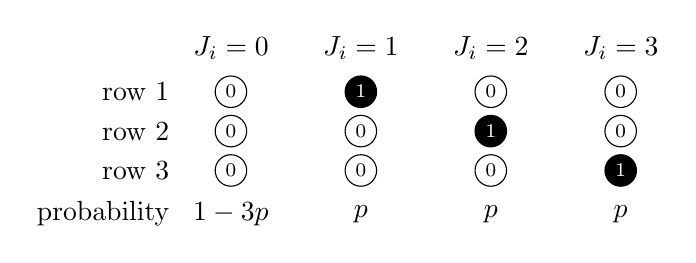
\begin{tikzpicture}[x=1.65cm,y=0.5cm,
  bit/.style={circle,draw,minimum size=4mm,inner sep=0pt},
  present/.style={bit,fill=black,text=white}]
  \foreach \x/\y in {0/1,0/2,0/3,1/1,1/2,2/1,2/3,3/2,3/3}
    \node[bit] at (\x,\y) {\scriptsize 0};
  \foreach \x/\y in {1/3,2/2,3/1}
    \node[present] at (\x,\y) {\scriptsize 1};
  \node at (0,4.1) {$J_i=0$};
  \node at (1,4.1) {$J_i=1$};
  \node at (2,4.1) {$J_i=2$};
  \node at (3,4.1) {$J_i=3$};
  \node at (0,-0.1) {$1-3p$};
  \foreach \x in {1,2,3} {\node at (\x,-0.1) {$p$};}
  \node[anchor=east] at (-0.4,3) {row 1};
  \node[anchor=east] at (-0.4,2) {row 2};
  \node[anchor=east] at (-0.4,1) {row 3};
  \node[anchor=east] at (-0.4,-0.1) {probability};
\end{tikzpicture}
\caption{One coordinate of the sparse coupling, illustrated with three
rows and $3p<1$. Each column is one possible value of the label $J_i$ and
shows which rows then contain coordinate $i$. Each row contains it with
probability $p$; the union contains it with probability $3p$. Making these
choices independently across coordinates gives the required product laws.}
\label{fig:coupling}
\end{figure}

\step{1.2}{the family $\mathcal F$ has $\mu_q$-measure at least $1/2$}
Define
\[
\mathcal F
=\{D_1\cup\cdots\cup D_L:D_1,\ldots,D_L\in\mathcal D\}.
\]
On the event in~\eqref{eq:all-good-rows}, $R=R_1\cup\cdots\cup R_L$ is a
union of $L$ members of $\mathcal D$, so $R\in\mathcal F$. Since $R$ has
law $\mu_q$,
\[
\mu_q(\mathcal F)=\mathbb P(R\in\mathcal F)
\ge\frac{31}{32}\ge\frac12.
\]

\step{1.3}{$E_{32}(\mathcal F)=E_k(\mathcal D)$}
The sets of the form $F_1\cup\cdots\cup F_{32}$ with $F_j\in\mathcal F$
are exactly the sets of the form $D_1\cup\cdots\cup D_{32L}$ with
$D_j\in\mathcal D$. In one direction, write each $F_j$ as a union of $L$
members of $\mathcal D$ and concatenate. In the other, split a
$32L$-tuple into $32$ consecutive blocks of length $L$; the union of each
block is in $\mathcal F$. By \eqref{eq:exceptional-definition},
\[
E_{32}(\mathcal F)=E_{32L}(\mathcal D)=E_k(\mathcal D).
\]

\step{1.4}{conclusion of Case 1}
By Step~1.2, Proposition~\ref{prop:half-density} applies to $\mathcal F$
at density $q$ and shows that $E_{32}(\mathcal F)$ is $(q/L)$-small. Since
$q/L=p$ and $E_{32}(\mathcal F)=E_k(\mathcal D)$, the family
$E_k(\mathcal D)$ is $p$-small.

\medskip
\noindent\emph{Case 2: $Lp\ge1$.} The labels of Case~1 are unavailable
because $1-Lp$ would be negative or zero, so a different coupling is used.

\step{2.1}{the coupling}
Set
\[
\tau=\frac{p-1/L}{1-1/L}.
\]
Then $\tau\ge0$ because $p\ge1/L$, and $\tau<1$ because $p<1$. For each
coordinate $i$, independently across coordinates: choose a ``mandatory''
row $K_i$ uniformly in $\{1,\ldots,L\}$; put $i$ into $R_{K_i}$; and,
conditionally on $K_i$, put $i$ into each other row independently with
probability $\tau$. For a fixed row $j$,
\[
\mathbb P(i\in R_j)
=\mathbb P(K_i=j)+\mathbb P(K_i\ne j)\,\tau
=\frac1L+\left(1-\frac1L\right)\tau=\frac1L+p-\frac1L=p,
\]
and the events $\{i\in R_j\}$, $i\in[N]$, are independent because the
choices at different coordinates are. So each $R_j$ has law $\mu_p$.
Moreover $R_1\cup\cdots\cup R_L=[N]$ in every outcome, since
$i\in R_{K_i}$.

\step{2.2}{conclusion of Case 2}
By~\eqref{eq:all-good-rows} the event that all $L$ rows lie in
$\mathcal D$ has positive probability, so it occurs for some outcome. This
gives $D_1,\ldots,D_L\in\mathcal D$ with $D_1\cup\cdots\cup D_L=[N]$.
Repeating this tuple $32$ times gives exactly $32L=k$ members of
$\mathcal D$ whose union is $[N]$, which contains every $S\subseteq[N]$.
By \eqref{eq:exceptional-definition}, $E_k(\mathcal D)=\varnothing$. The
empty family covers it at cost $0\le1/2$. The boundary case $Lp=1$ is
included, with $\tau=0$.
\end{proof}

\section{Consequences and context}
\label{sec:context}

Nothing in this section is used in the proof of Theorem~\ref{thm:main}.
Section~\ref{sec:selectors} is a self-contained consequence of the
theorem. Section~\ref{sec:two-union} is a separate result whose proof
depends on three cited papers. Section~\ref{sec:related} lists related
work as described in the original manuscript.

\subsection{Positive selector processes}
\label{sec:selectors}

The link between discrete convexity and positive selector processes is
explained in \cite[Section~7]{Talagrand10} and
\cite[Proposition~13.3.3]{Talagrand21}. Concretely, let
$\mathcal T\subseteq[0,\infty)^N$ be nonempty and define
\[
\phi(S)=\sup_{\theta\in\mathcal T}\sum_{i\in S}\theta_i\quad(S\subseteq[N]),
\qquad M=\mathbb E_{\mu_p}\phi,
\]
and suppose $0<M<\infty$.

\smallskip
\noindent\textbf{Claim.} \emph{With $k=2^{75}$, the family
$\{S:\phi(S)\ge k^2M\}$ is $p$-small.}

\smallskip
\noindent\emph{Proof.}
(1) Let $\mathcal D=\{D:\phi(D)<kM\}$. Since $\phi\ge0$ and $M>0$,
Markov's inequality gives $\mu_p\{\phi\ge kM\}\le1/k$, so
$\mu_p(\mathcal D)\ge1-1/k$.

(2) $\phi$ is monotone: if $A\subseteq B$ then $\phi(A)\le\phi(B)$,
because all $\theta_i\ge0$. And $\phi$ is subadditive under unions: for
every $\theta\in\mathcal T$,
$\sum_{i\in A\cup B}\theta_i\le\sum_{i\in A}\theta_i+\sum_{i\in B}\theta_i
\le\phi(A)+\phi(B)$, and taking the supremum over $\theta$ gives
$\phi(A\cup B)\le\phi(A)+\phi(B)$.

(3) If $S\subseteq D_1\cup\cdots\cup D_k$ with all $D_j\in\mathcal D$,
then by (2) $\phi(S)\le\sum_{j=1}^k\phi(D_j)<k\cdot kM$. Hence
$\{S:\phi(S)\ge k^2M\}\subseteq E_k(\mathcal D)$.

(4) By (1), Theorem~\ref{thm:main} gives a cover of $E_k(\mathcal D)$ of
cost at most $1/2$ at density $p$. By (3) it also covers
$\{S:\phi(S)\ge k^2M\}$. \qed

\smallskip
The original manuscript notes that this recovers the positive-selector
conclusion proved by Park and Pham \cite[Theorem~1.2]{ParkPham24}, a
statement of the same shape (the set where $\phi$ exceeds a universal
constant multiple of $M$ is $p$-small), here with the constant
$k^2=2^{150}$. As for what the claim adds: Markov's inequality alone
bounds only the probability, $\mu_p\{\phi\ge k^2M\}\le k^{-2}$. The claim
supplies a structural certificate of a different kind, namely an explicit
list $\mathcal G$ of sets with $\sum_{I\in\mathcal G}p^{|I|}\le1/2$ such
that every $S$ with $\phi(S)\ge k^2M$ contains a member of $\mathcal G$.

\subsection{Two unions at constant density loss}
\label{sec:two-union}

Theorem~\ref{thm:main} keeps the density $p$ but uses $2^{75}$ unions and
needs $\mu_p(\mathcal D)\ge1-2^{-75}$. The following corollary
(Corollary~1.2 of the original manuscript) sits at the other end of the
tradeoff: two unions, hypothesis $\mu_p(\mathcal D)>1/2$, and a constant
factor lost in the density. Its proof does not use
Sections~\ref{sec:covering}--\ref{sec:density}; it combines external
results.

\paragraph{Fractional smallness.}
For $\sigma\in(0,1)$, a family $\mathcal A$ has a \emph{fractional cover
of cost at most $1/2$ at density $\sigma$} if there are coefficients
$a_I\ge0$ ($I\subseteq[N]$) with
\[
\sum_{I\subseteq S}a_I\ge1\quad(S\in\mathcal A),
\qquad
\sum_{I\subseteq[N]}\sigma^{|I|}a_I\le\frac12.
\]
A cover in the sense of Section~\ref{sec:introduction} is the special case
$a_I\in\{0,1\}$; it is called \emph{integral} below. Talagrand introduced
this relaxation alongside integral
smallness~\cite[Sections~6 and~7]{Talagrand10}.

\paragraph{The cited inputs, in the form the proof uses them.}
\begin{itemize}
\item[(I1)] \emph{Li's result \cite[Corollary~3.1]{Li26} in Park's
fractional-cover formulation \cite[Theorem~3.4]{Park26}.} As invoked: if
$\mu_p(\mathcal D)>1/2$ and $E_2(\mathcal D)$ is a nonempty proper
increasing family, then $E_2(\mathcal D)$ has a fractional cover of cost
at most $1/2$ at density $\sigma=p/2$.
\item[(I2)] \emph{The companion theorem
\cite[Theorem~1.1]{OpenAIThreshold26}.} The original manuscript calls it
both the ``companion constant-factor rounding theorem'' and the
``companion expectation-threshold theorem''; both refer to this one
citation. As invoked: a family as in (I1) that has a fractional cover of
cost at most $1/2$ at density $\sigma$, with all coefficients in $[0,1]$,
has an integral cover of cost at most $1/2$ at density
$\sigma/(25\cdot512^4)$.
\end{itemize}
Here ``proper'' is read as ``not all of $2^{[N]}$''. For an increasing
family this is the same as not containing $\varnothing$, which is what the
proof checks.

\begin{corollary}[Two unions at constant density loss]
\label{cor:two-union}
There is a universal constant $C\ge1$ such that, for every integer $N\ge1$,
every $p\in(0,1)$, and every family $\mathcal D\subseteq2^{[N]}$,
\[
\mu_p(\mathcal D)>\frac12
\quad\Longrightarrow\quad
E_2(\mathcal D)\text{ is }(p/C)\text{-small}.
\]
\end{corollary}

\begin{proof}
(1) If $E_2(\mathcal D)=\varnothing$, the empty cover suffices.

(2) Otherwise $E_2(\mathcal D)$ is nonempty. It is increasing by the
second bullet after \eqref{eq:exceptional-definition}. It is proper:
$\mu_p(\mathcal D)>0$ gives $\mathcal D\ne\varnothing$, so
$\varnothing\notin E_2(\mathcal D)$ by the first bullet there.

(3) By (I1), $E_2(\mathcal D)$ has a fractional cover $(a_I)$ of cost at
most $1/2$ at density $\sigma=p/2$.

(4) Replace each $a_I$ by $a_I'=\min\{a_I,1\}$. The cost does not
increase. Coverage is preserved: for $S\in E_2(\mathcal D)$, if some
$I\subseteq S$ has $a_I\ge1$ then $\sum_{I\subseteq S}a'_I\ge1$, and
otherwise the sum is unchanged.

(5) By (I2) there is an integral cover of cost at most $1/2$ at density
$\sigma/(25\cdot512^4)=p/(50\cdot512^4)$. Thus $C=50\cdot512^4$ suffices.
\end{proof}

\unverified{Steps (3) and (5) rest on (I1) and (I2), which are quoted
above in the form in which the original manuscript uses them. That
manuscript does not reproduce the statements of
\cite[Corollary~3.1]{Li26}, \cite[Theorem~3.4]{Park26} and
\cite[Theorem~1.1]{OpenAIThreshold26}. I could not check that their
hypotheses are met by $E_2(\mathcal D)$ under $\mu_p(\mathcal D)>1/2$, why
the density is $p/2$, or the constant $25\cdot512^4$. A natural guess,
not confirmed, is that the factor $2$ arises when a statement about
probability measures with containment probabilities at most $p^{|I|}$ is
dualised into a fractional cover of cost $1/2$, since
$2(p/2)^{|I|}\le p^{|I|}$ for $|I|\ge1$. Steps (1), (2), (4) and the
arithmetic in (5) are verified. The corollary is not used for
Theorem~\ref{thm:main}.}

\paragraph{Which citation is which.}
The original manuscript cites four different statements from
\cite{Li26} and \cite{Park26}. Its descriptions are as follows.
\cite[Theorem~1.9]{Li26} resolves the fractional discrete-convexity
problem through a quantitative obstruction to probability measures whose
containment probabilities are bounded by $p^{|I|}$; it is cited as
context. \cite[Corollary~3.1]{Li26} and \cite[Theorem~3.4]{Park26} are the
forms invoked in (I1). \cite[Corollary~3.5]{Park26} is Park's own integral
result: combining fractional information with rounding, Park obtains an
integral cover of $E_2(\mathcal D)$ at density
\[
\frac{p}{C\max\{1,\log\log(1/p)\}}
\]
whenever $\mu_p(\mathcal D)>1/2$, for a universal $C$.
Corollary~\ref{cor:two-union} has the same hypothesis and replaces this
density by $p/C$. In the manuscript's account, the difference lies in
using the constant-factor rounding theorem (I2) for the rounding step.

\subsection{Related developments}
\label{sec:related}

The following descriptions are those of the original manuscript.

\paragraph{Origin of the name.}
The name reflects the analogy with Talagrand's Gaussian convexity
question~\cite[Conjecture~2.1]{Talagrand10}: can a bounded number of
sums of a compact balanced set of sufficiently large Gaussian measure
contain a convex set of Gaussian measure at least $1/2$, uniformly in
the dimension? Here balanced means closed under multiplication by
scalars of absolute value at most one. In the discrete problem, unions
replace sums, and containment covers describe the exceptional sets.

\paragraph{Other results.}
Hua, Song, and Tudose resolve Talagrand's Gaussian convexity problem and
derive a discrete conclusion with three unions and covering density
$p^C$, for a universal constant $C$, when the starting family is
sufficiently likely~\cite[Corollaries~1.3--1.4]{HuaSongTudose26}.
Ascoli, He, Park, and Talagrand give a threshold reformulation of discrete
convexity and prove cases for several graph-containment
properties~\cite[Proposition~1.5 and Theorems~1.10--1.13]{AscoliEtAl26}.

\paragraph{Antecedents of the method.}
The signed product of Step~2 of Proposition~\ref{prop:half-density} has
antecedents in the signed product operators and biased Fourier analysis of
Friedgut~\cite[Section~2.2]{Friedgut08} and Ellis, Filmus, and
Friedgut~\cite[Sections~2.2 and~4.1]{EllisFilmusFriedgut12}. Its two-row
version is attributed to Li~\cite[Section~2]{Li26}. Random unions also
enter the covering constructions of Fischer and
Person~\cite[Sections~1.1 and~2]{FischerPerson25}.

\section{Verification checklist}
\label{sec:checklist}

A sceptical reader should check these load-bearing steps first.

\begin{enumerate}
\item \textbf{Extension inequality \eqref{eq:covering-extension}}
(Lemma~\ref{lem:covering}, Step~2). Check that a nonempty group
$\{e\in\mathcal H':e\cap B=I\}$ forces $d(I)\le T$, and that the number of
groups is at most $\sum_{i\le r}\binom{|B|}{i}$. This inequality drives
both the pair cost \eqref{eq:covering-pair-cost} and the recursion
\eqref{eq:W-recursion}.
\item \textbf{Survival probability and arithmetic}
(Lemma~\ref{lem:covering}, Steps~5b--5c). The $m^2$ pairs of a tuple of
distinct edges are distinct sampling indices, diagonal included, giving
$(1-\pi)^{m^2}$. Then check $4h+13rh+1\le2^{4h}=\pi m$, which uses
$r\le h$ and $h\ge3$.
\item \textbf{$\mathcal G$ is a cover for every outcome}
(Lemma~\ref{lem:covering}, Step~4). Every edge inside a set avoiding
$\mathcal C_0$ is regular, and the dichotomy ``some pair sampled / no pair
sampled'' is exhaustive.
\item \textbf{Normalization
$\widehat f(U)=(q/(1-q))^{|U|/2}b(U)$ and (W1)}
(Proposition~\ref{prop:half-density}, Step~1b--1c).
\item \textbf{Signed identity \eqref{eq:signed-identity}}
(Proposition~\ref{prop:half-density}, Step~2). Two points:
$\widetilde P(0,\ldots,0)=0$ makes every term of $\Sigma$ vanish (2b),
and the $U$-term factors over the $32$ rows with each row giving exactly
$b(U)$ (2c).
\item \textbf{Bin bookkeeping}
(Proposition~\ref{prop:half-density}, Steps~4--6). Nonempty bins have
$h\ge64r$; $|\mathcal H_{r,h}|\rho^r\le2^{h+1}$; the two geometric sums
\eqref{eq:bin-cost-sum} and \eqref{eq:bin-power-sum}; and the comparison
$16/(15(2^{256}-1))<2^{-32}\le$ the bound
\eqref{eq:exceptional-weight-bound}.
\item \textbf{The couplings} (Section~\ref{sec:density}). In Case~1 each
row has law exactly $\mu_p$, the union has law exactly $\mu_{Lp}$, and
$E_{32}(\mathcal F)=E_{32L}(\mathcal D)$ (Steps~1.1--1.3). In Case~2 each
row has law $\mu_p$ and the rows always cover $[N]$ (Step~2.1).
\item \textbf{Scope.} Corollary~\ref{cor:two-union} depends on the
external inputs (I1) and (I2), which are not verified here (see the box in
Section~\ref{sec:two-union}). Theorem~\ref{thm:main} does not depend on
it.
\end{enumerate}

\begin{thebibliography}{99}

\bibitem{AscoliEtAl26}
Ruben Ascoli, Xiaoyu He, Jinyoung Park, and Michel Talagrand,
\emph{A reformulation of the discrete Convexity Conjecture via
$k$-thresholds},
arXiv:2608.11183v1, 2026.
\href{https://arxiv.org/abs/2608.11183v1}{arXiv:2608.11183v1}.

\bibitem{EllisFilmusFriedgut12}
David Ellis, Yuval Filmus, and Ehud Friedgut,
\emph{Triangle-intersecting families of graphs},
Journal of the European Mathematical Society \textbf{14} (2012),
no.~3, 841--885.
\href{https://doi.org/10.4171/JEMS/320}{doi:10.4171/JEMS/320}.

\bibitem{FischerPerson25}
Thomas Fischer and Yury Person,
\emph{Further remarks on fractional vs. expectation thresholds},
arXiv:2505.21782v1, 2025.
\href{https://doi.org/10.48550/arXiv.2505.21782}{doi:10.48550/arXiv.2505.21782}.

\bibitem{Friedgut08}
Ehud Friedgut,
\emph{On the measure of intersecting families, uniqueness and stability},
Combinatorica \textbf{28} (2008), no.~5, 503--528.
\href{https://doi.org/10.1007/s00493-008-2318-9}{doi:10.1007/s00493-008-2318-9}.

\bibitem{HuaSongTudose26}
Dongming (Merrick) Hua, Antoine Song, and Stefan Tudose,
\emph{On Talagrand's Convexity Conjecture},
arXiv:2605.10908v2, 2026.
\href{https://arxiv.org/abs/2605.10908v2}{arXiv:2605.10908v2}.

\bibitem{Li26}
Chen Li,
\emph{On $p$-spread measures},
arXiv:2609.08967v1, 2026.
\href{https://arxiv.org/abs/2609.08967v1}{arXiv:2609.08967v1}.

\bibitem{ODonnell14}
Ryan O'Donnell,
\emph{Analysis of Boolean Functions},
Cambridge University Press, Cambridge, 2014.
Author's corrected text, 2021:
\href{https://arxiv.org/abs/2105.10386v1}{arXiv:2105.10386v1}.

\bibitem{OpenAIThreshold26}
OpenAI,
\emph{Integral and fractional expectation thresholds are equivalent},
OpenAI Math Release preprint
\href{https://github.com/openai/math/blob/main/preprints/Integral-and-fractional-expectation-thresholds-are-equivalent-September-23-2026/paper.pdf}{OAI:Integral-and-fractional-expectation-thresholds-are-equivalent-September-23-2026},
2026.

\bibitem{Park26}
Jinyoung Park,
\emph{A dimension-free comparison between expectation thresholds and
fractional expectation thresholds},
arXiv:2609.14681v1, 2026.
\href{https://arxiv.org/abs/2609.14681v1}{arXiv:2609.14681v1}.

\bibitem{ParkPham24}
Jinyoung Park and Huy Tuan Pham,
\emph{On a conjecture of Talagrand on selector processes and a consequence
on positive empirical processes},
Annals of Mathematics \textbf{199} (2024), no.~3, 1293--1321.
\href{https://doi.org/10.4007/annals.2024.199.3.6}{doi:10.4007/annals.2024.199.3.6}.

\bibitem{Talagrand10}
Michel Talagrand,
\emph{Are many small sets explicitly small?},
Proceedings of the Forty-Second ACM Symposium on Theory of Computing,
ACM, New York, 2010, 13--36.
\href{https://doi.org/10.1145/1806689.1806693}{doi:10.1145/1806689.1806693}.

\bibitem{Talagrand21}
Michel Talagrand,
\emph{Upper and Lower Bounds for Stochastic Processes:
Decomposition Theorems},
2nd ed., Ergebnisse der Mathematik und ihrer Grenzgebiete, 3.~Folge,
vol.~60, Springer, Cham, 2021.
\href{https://doi.org/10.1007/978-3-030-82595-9}{doi:10.1007/978-3-030-82595-9}.

\end{thebibliography}

\end{document}
